% fig_freq_correction_error.tex
% Bar + line chart: residual charging error (ε_C) vs frequency
% Fixed (TR-15) vs Adaptive (TR-20) — Study A results
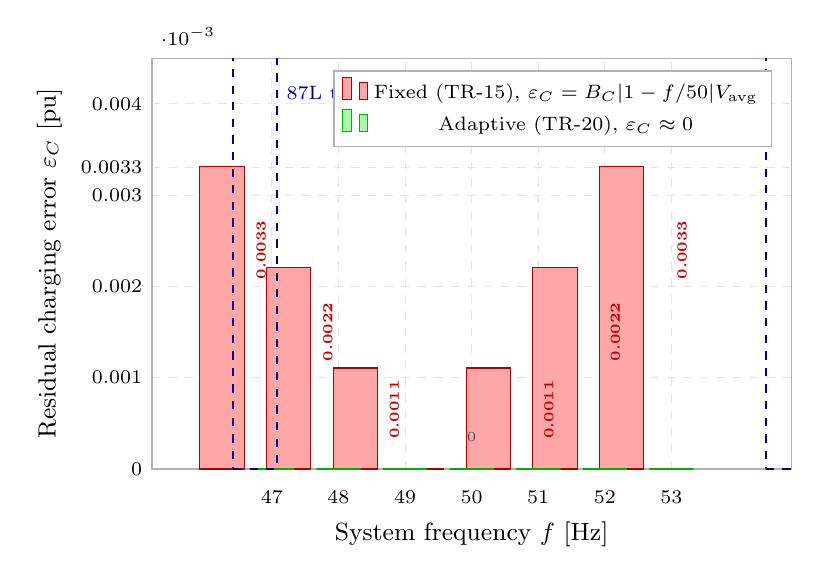
\begin{tikzpicture}
\begin{axis}[
  name         = fceax,
  ybar,
  bar width    = 16pt,
  width        = 0.80\textwidth,
  height       = 6.8cm,
  ylabel       = {Residual charging error $\varepsilon_C$ [pu]},
  ylabel style = {font=\small},
  xlabel       = {System frequency $f$ [Hz]},
  xlabel style = {font=\small},
  ymin=0, ymax=0.0045,
  ytick        = {0, 0.001, 0.002, 0.003, 0.0033, 0.004},
  yticklabels  = {0, 0.001, 0.002, 0.003, 0.0033, 0.004},
  yticklabel style={font=\scriptsize},
  xtick        = {47, 48, 49, 50, 51, 52, 53},
  xticklabels  = {47, 48, 49, 50, 51, 52, 53},
  xticklabel style={font=\scriptsize},
  enlarge x limits=0.10,
  legend style={at={(0.97,0.97)}, anchor=north east,
                font=\scriptsize, draw=gray!60},
  grid          = major,
  grid style    = {gray!20, dashed},
  tick style    = {draw=none},
  axis line style={gray!60},
]

% Fixed (TR-15) residuals — eps = B_C * |1 - f/50| * V_rms (approx)
\addplot[fill=red!35, draw=red!70!black]
  coordinates {
    (47, 0.003312)
    (48, 0.002210)
    (49, 0.001106)
    (50, 0.000000)
    (51, 0.001106)
    (52, 0.002210)
    (53, 0.003313)
  };
\addlegendentry{Fixed (TR-15), $\varepsilon_C = B_C|1-f/50|V_{\rm avg}$}

% Adaptive (TR-20) residuals — all ≈ 0
\addplot[fill=green!35, draw=green!70!black]
  coordinates {
    (47, 0.0)
    (48, 0.0)
    (49, 0.0)
    (50, 0.0)
    (51, 0.0)
    (52, 0.0)
    (53, 0.0)
  };
\addlegendentry{Adaptive (TR-20), $\varepsilon_C \approx 0$}

% ---- Value annotations (Fixed only, adaptive all ~0) -------------------
\node[font=\tiny\bfseries, red!80!black, rotate=90]
  at (axis cs:46.84, 0.0024) {0.0033};
\node[font=\tiny\bfseries, red!80!black, rotate=90]
  at (axis cs:47.84, 0.0015) {0.0022};
\node[font=\tiny\bfseries, red!80!black, rotate=90]
  at (axis cs:48.84, 0.00065) {0.0011};
\node[font=\tiny, gray!60!black, rotate=0]
  at (axis cs:50.0, 0.00035) {0};
\node[font=\tiny\bfseries, red!80!black, rotate=90]
  at (axis cs:51.16, 0.00065) {0.0011};
\node[font=\tiny\bfseries, red!80!black, rotate=90]
  at (axis cs:52.16, 0.0015) {0.0022};
\node[font=\tiny\bfseries, red!80!black, rotate=90]
  at (axis cs:53.16, 0.0024) {0.0033};

% ---- 87L threshold annotation ------------------------------------------
\addplot[blue!60!black, thick, dashed, mark=none, domain=46:54, samples=2]
  ({x}, {0.12});   % threshold far above — annotation only
% (Threshold at 0.12 pu is off-chart; show note instead)
\node[font=\scriptsize, blue!60!black, align=center]
  at (axis cs:50.0, 0.0041)
  {87L threshold at 0.12\,pu $\gg$ axis range};

\end{axis}
\end{tikzpicture}
